\documentclass{article}
\usepackage[utf8]{inputenc}
\usepackage{amsmath}
\usepackage{mathtools}
\usepackage{amsthm}
\usepackage{graphicx}
\usepackage{tabularx}
\usepackage{mathtools}
\usepackage{mathrsfs}
\usepackage{enumerate}
\usepackage{amssymb}
\usepackage{accents}
\usepackage{commath}
\usepackage{yfonts}
\usepackage{float}
\usepackage{array}
\usepackage{tikz-cd}
\usepackage{listings}

\title{Stat3004 Assignment 3}
\author{Dominic Scocchera}
\date{April 2023}

\newtheorem{theorem}{Theorem}
\newtheorem{corollary}{Corollary}
\newtheorem{lemma}[theorem]{Lemma}

\begin{document}
\maketitle
%https://math.stackexchange.com/questions/2172959/joint-mass-function-of-a-poisson-process
\section*{Q1}
First we note that $N((a,b])\sim Poi(2\cdot(b-a))$.
\subsection*{a)}
\begin{align*}
\mathbb{P}(N_{t_1}=n_1,N_{t_2}=n_2)&=\mathbb{P}(N_{2}=7,N_{12}=10)\\
&=\mathbb{P}(N_2=7,N_{12-2}=10-7)\\
&=\mathbb{P}(N_2=7)\mathbb{P}(N_{10}=3)\\
&=e^{-2\cdot2}\frac{(2\cdot2)^7}{7!}e^{-2\cdot10}\frac{(2\cdot10)^{3}}{3!}\\
&\approx1.636291121\times10^{-7}\\
\end{align*}
\subsection*{b)}
\begin{align*}
\mathbb{P}(N(1, t_1]=n_1, N(t_1-1,t_2]=n_2)&=\mathbb{P}(N(1,2]=7, N(1,12]=10)\\
&=\mathbb{P}(N(1,2]=7, N(2,12]=3)\\
&=\mathbb{P}(N(1,2]=7)\mathbb{P}(N(2,12]=3)\\
&=\frac{e^{-2}(2)^7}{7!}\frac{e^{-20}(20)^3}{3!}\\
&\approx 9.4458178806\times10^{-9}\\
\end{align*}
\subsection*{c)}
\begin{align*}
\mathbb{E}[N(1,t_1]\;|\;N(t_1-1,t_2]=n_2]&=\mathbb{E}[N(1,2]\;|\;N(1,12]=10]\\
&=\sum_{t\geq0}t\cdot\mathbb{P}(N(1,2]=t|N(1,12]=10)\\
&=\sum_{t=0}^{10}t\cdot\frac{\mathbb{P}(N(1,2]=t,N(1,12]=10)}{\mathbb{P}(N(1,12]=10)}\\
&=\frac{1}{\mathbb{P}(N(1,12]=10)}\sum_{t=0}^{10}t\cdot\mathbb{P}(N(1,2]=t,N(2,12]=10-t)\\
&=\frac{1}{\mathbb{P}(N(1,12]=10)}\sum_{t=0}^{10}t\cdot\mathbb{P}(N(1,2]=t)\mathbb{P}(N(2,12]=10-t)\\
&=\frac{1}{\frac{e^{-22}(22)^{10}}{10!}}\sum_{t=0}^{10}t\cdot\frac{e^{-2}(2)^t}{t!}\frac{e^{-20}(20)^{10-t}}{(10-t)!}\\
&=\frac{1}{(22)^{10}}\sum_{t=0}^{10}{10 \choose t}t\cdot(2)^t(20)^{10-t}\\
&=\frac{24145384355840}{22^{10}}\\
&=\frac{10}{11}\\
\end{align*}
\subsection*{d)}
\begin{align*}
\mathbb{E}[N(t_1-1,t_2]\;|\;N(1,t_1]=n_1]&=\mathbb{E}[N(1,12]\;|\;N(1,2]=7]\\
&=\sum_{t\geq0}t\cdot\mathbb{P}(N(1,12]=t|N(1,2]=7)\\
&=\sum_{t\geq7}t\cdot\mathbb{P}(N(1,12]=t|N(1,2]=7)\\
&=\sum_{t\geq7}t\cdot\frac{\mathbb{P}(N(1,12]=t,N(1,2]=7)}{\mathbb{P}(N(1,2]=7)}\\
&=\sum_{t\geq7}t\cdot\frac{\mathbb{P}(N(2,12]=t-7)\mathbb{P}(N(1,2]=7)}{\mathbb{P}(N(1,2]=7)}\\
&=\sum_{t\geq7}t\cdot\mathbb{P}(N(2,12]=t-7)\\
&=\sum_{t\geq7}t\cdot\frac{e^{-20}20^{t-7}}{(t-7)!}\\
&=\sum_{x\geq0}(x+7)\cdot\frac{e^{-20}20^{x}}{x!},\;\;\;\text{note }x=t-7\\
&=\sum_{x\geq0}x\cdot\frac{e^{-20}20^{x}}{x!}+7\sum_{x\geq0}\frac{e^{-20}20^{x}}{x!}\\
&=\mathbb{E}[x]+7\cdot1,\;\;\;x\sim Poi(20)\\
&=20+7\\
&=27\\
\end{align*}
\section*{Q2}
First note that $N_{t+s}-N_{t}\sim Poi\left(\int_{t}^{t+s}\lambda(t)dt\right)$
\begin{align*}
\mathbb{P}(N_{s}=m|N_{t}=n)&=\frac{\mathbb{P}(N_{s}=m,N_{t}=n)}{\mathbb{P}(N_{t}=n)}\\
&=\frac{\mathbb{P}(N_{s}=m,N_{t}-N_{s}=n-m)}{\mathbb{P}(N_{t}=n)}\\
&=\frac{\mathbb{P}(N_{s}=m)\mathbb{P}(N_{t}-N_{s}=n-m)}{\mathbb{P}(N_{t}=n)}\\
&=\frac{\frac{\left(\int_{0}^{s}1-e^{-t}dt\right)^me^{-\int_{0}^{s}1-e^{-t}dt}}{m!}\frac{\left(\int_{s}^{t}1-e^{-t}dt\right)^{n-m}e^{-\int_{s}^{t}1-e^{-t}dt}}{(n-m)!}}{\frac{\left(\int_{0}^{t}1-e^{-t}dt\right)^ne^{-\int_{0}^{t}1-e^{-t}dt}}{n!}}\\
&=\frac{n!(s-1+e^{-s})^me^{1-s-e^{-s}}(t-s+e^{-t}-e^{-s})^{n-m}e^{t-s+e^{-t}-e^{-s}}}{m!(n-m)!(t-1+e^{-t})^ne^{1-t-e^{-t}}}\\
&={n\choose m}e^{2e^{-t}-2e^{-s}+2t-2s}\frac{(s-1+e^{-s})^m(t-s+e^{-t}-e^{-s})^{n-m}}{(t-1+e^{-t})^n}\\
\end{align*}
\section*{Q3}
\subsection*{a)}
First we have that $N_A\sim Poi(\lambda|A|)=Poi(0.5\cdot0.25)=Poi(1/8)$.
\begin{align*}
\mathbb{P}(N_A\geq1)&=1-\mathbb{P}(N_A=0)\\
&=1-\frac{e^{-\frac{1}{8}}\left(\frac{1}{8}\right)^0}{0!}\\
&=1-e^{-\frac{1}{8}}\\
&\approx 0.1175\\
\end{align*}
\subsection*{b)}
As each trip explores a new area we have that each trip is an independent Poisson process. This means if make n trips we have the Poisson process $\sum_{i=1}^{n}N_{i}\sim Poi(\sum_{i=1}^{n}\lambda|A|)=Poi(n\lambda|A|)$. So the expectation is $\mathbb{E}[\sum_{i=1}^{n}N_{i}]=n\lambda|A|=\frac{n}{8}$. Now we want to find the n that makes this greater or equal to 6, thus $n=48$ ($\frac{48}{8}=6$). Therefore we can expect to make 48 trips before we see 6 fat-tailed dunnarts. 
\subsection*{c)}
If we assume the survey was also a spatial Poisson process with the same rate parameter, let A be the event that there are a total of $5\cdot10^5$ fat-tailed dunnarts over the total $29750km^2$. We then have:
$$\mathbb{P}(A)=\frac{e^{-0.5\cdot29750}(0.5\cdot29750)^{5\cdot10^5}}{(5\cdot10^5)!}$$
\begin{align*}
\mathbb{P}(N_{A}\geq1|A)&=1-\mathbb{P}(N_{A}=0|A)\\
&=1-\frac{\mathbb{P}(N_{A}=0,A)}{\mathbb{P}(A)}\\
\end{align*}
\section*{Q4}
\subsection*{a)}
We have four states for this problem:
\begin{align*}
0:&\text{Both machines are functioning}\\
1:&\text{The machine has failed, but the repair robot is functioning}\\
2:&\text{The repair robot has failed, but the machine is functioning}\\
3:&\text{Both machines have failed}\\
\end{align*}
So $E=\{0,1,2,3\}$. We know that both machines initially are working, so $\pi^{(0)}=(1,0,0,0)^T$. Now noting the given lifetime and repair distributions and that we can't have an infitesimal change between state 1 and 2, 0 and 3, and, we can't go from state 3 to 2 as the repair robot needs to be repaired before the machine we get that the $Q$-matrix is:
$$Q=\begin{pmatrix}
-108 & 4 & 104 & 0\\
1 & -105 & 0 & 104\\
26 & 0 & -30 & 4\\
0 & 26 & 0 & -26\\
\end{pmatrix}$$
\subsection*{b)}
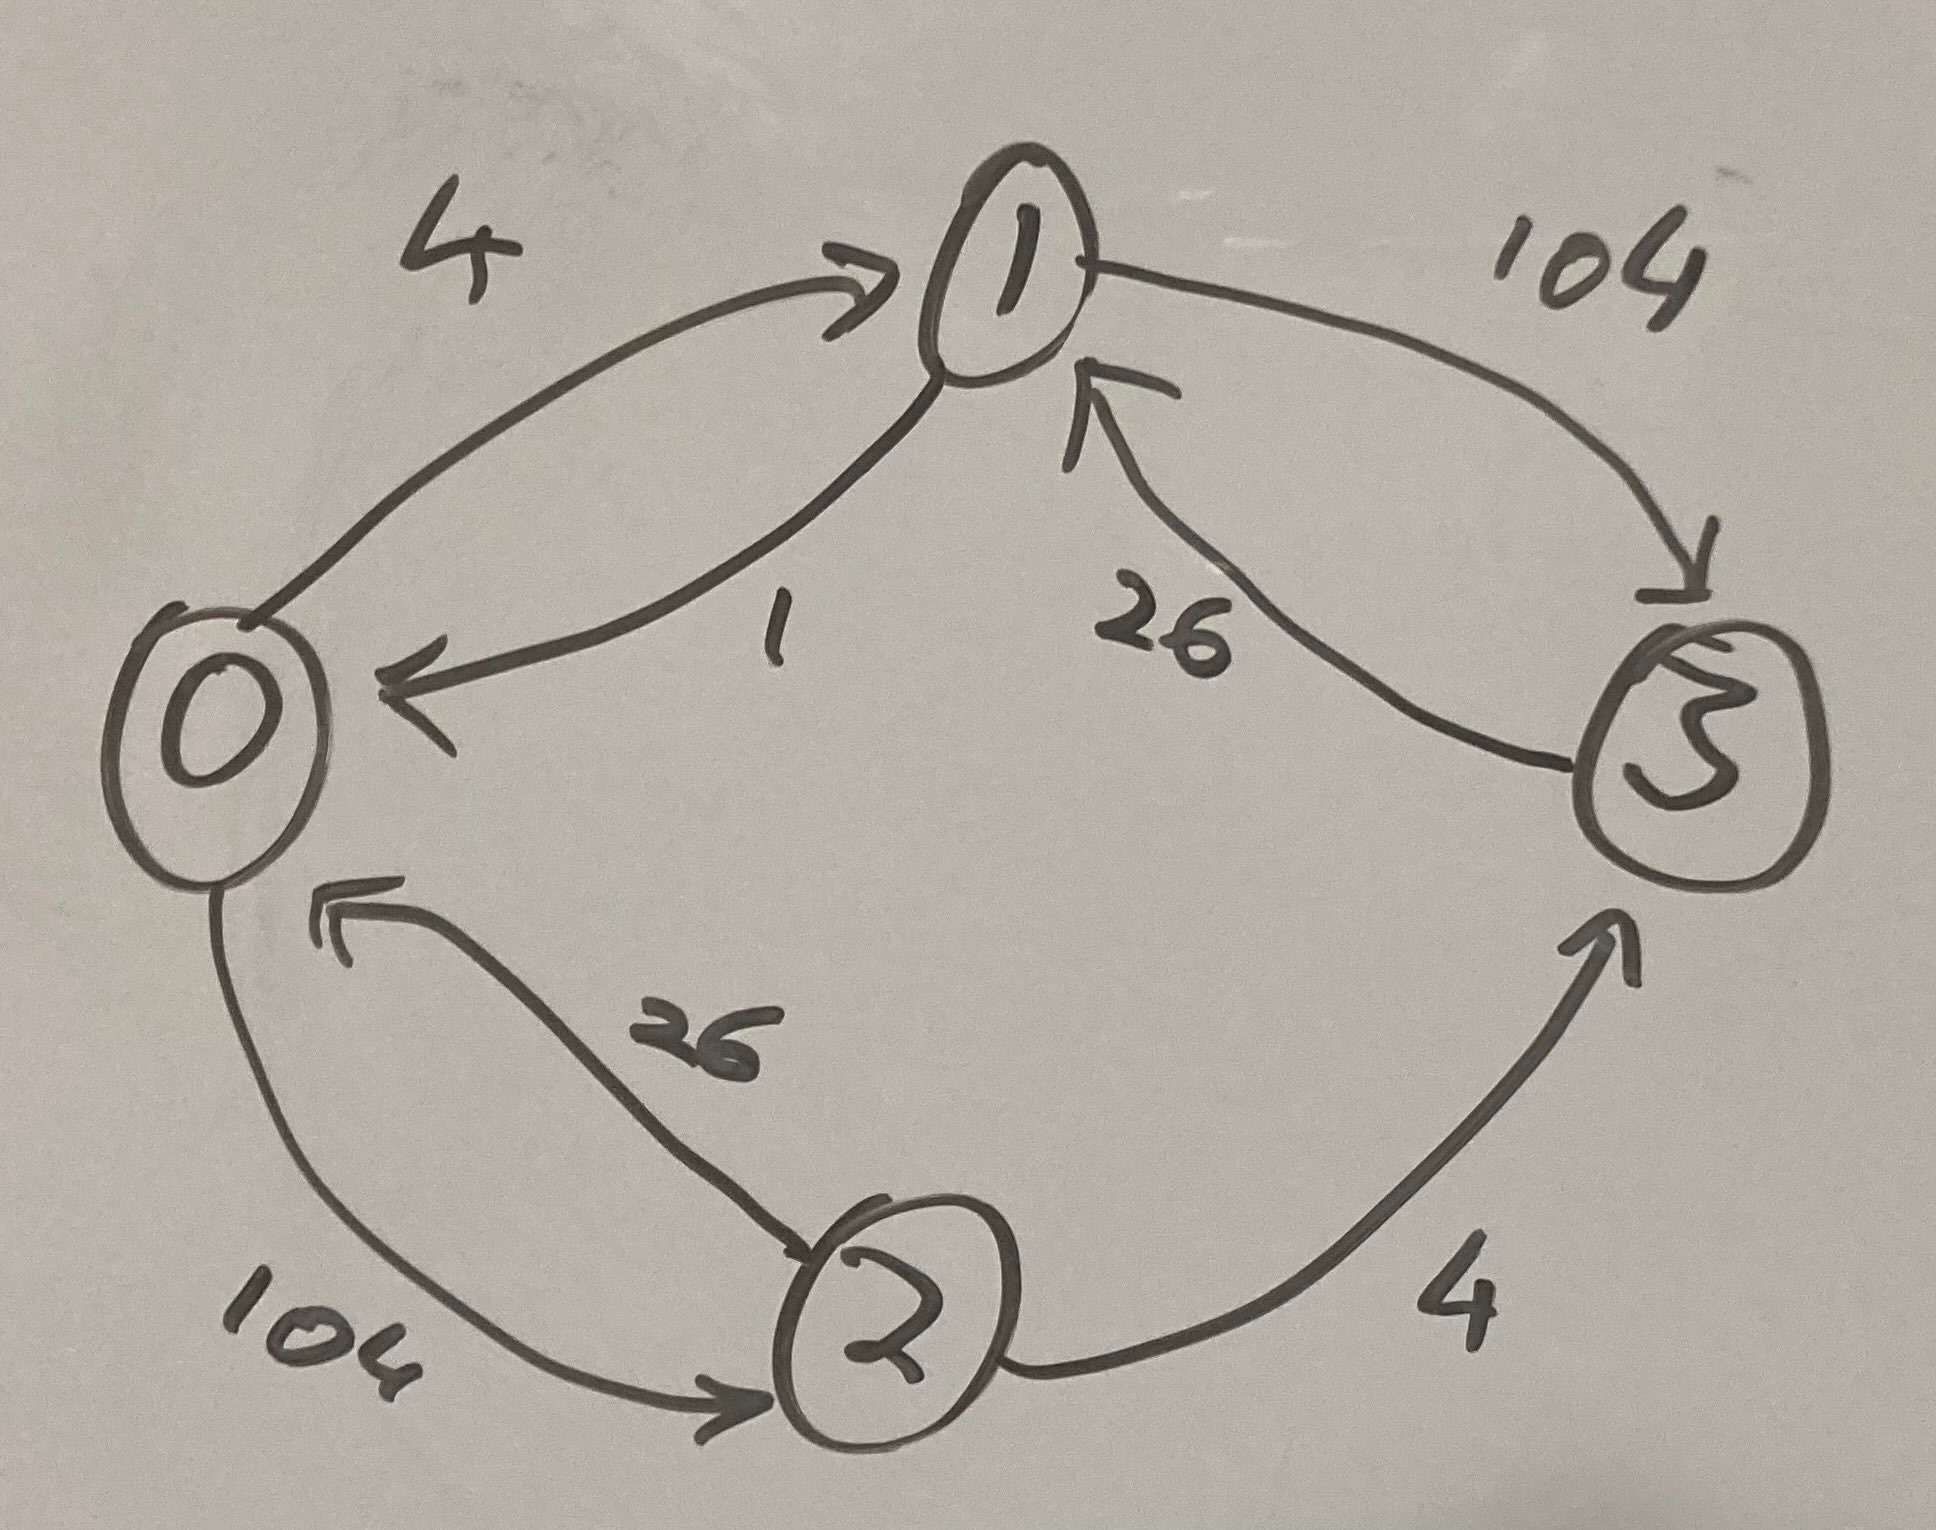
\includegraphics[scale=0.2]{CTMC.jpeg}
\subsection*{c)}
We calculate the long run distribution $\pi$ by solving $\pi Q=\bold{0}$ such that $\pi\bold{1}=1$.
\begin{align*}
0&=104\pi_0-30\pi_2\implies \pi_0=\frac{15}{52}\pi_2\;\;\;(1)\\
0&=-108\pi_0+\pi_1+26\pi_2\implies\pi_1=108\pi_0-26\pi_2=(\frac{3240}{104}-26)\pi_2=\frac{67}{13}\pi_2\;\;\;(2)\\
0&=4\pi_0-105\pi_1+26\pi_3\implies\pi_3=\frac{105\pi_1-4\pi_0}{26}=\frac{270}{13}\pi_2\;\;\;(3)\\
1&=\pi_0+\pi_1+\pi_2+\pi_3\implies \frac{1}{\frac{15}{52}+\frac{67}{13}+1+\frac{270}{13}}=\pi_2=\frac{52}{1415}\;\;\;(4)\\
\end{align*}
Subbing (4) into (1), (2) and (3) we get:
$$\pi=\left(\frac{3}{283},\frac{268}{1415},\frac{52}{1415},\frac{216}{283}\right)^T$$
So the long run probability that both the machine and the machine repair
robot are under repair is $\frac{216}{283}$.
\subsection*{d)}
To find the this probability we first find the transition matrix of the embedded markov chain (D), where the entry $d_{ij}=\frac{q_{ij}}{-q_{ii}}$, where $q_{ij}$ are entries from the $Q$-matrix.
$$D=\begin{pmatrix}
0 & \frac{4}{108} & \frac{104}{108} & 0\\
\frac{1}{105} & 0 & 0 & \frac{104}{105}\\
\frac{26}{30} & 0 & 0 & \frac{4}{30}\\
0 & 1 & 0 & 0\\
\end{pmatrix}$$
If the machine has failed and is under repair we are in state 1 and the probability that it transitions to 0 and not 3 is from the matrix D, $\frac{1}{105}$.
\end{document}